\documentclass{article}
\usepackage{ctex}
\usepackage{setspace}
\usepackage{float}
\usepackage{booktabs}
\usepackage{listings} %和代码框有关的两个宏包
\usepackage{xcolor}
\usepackage{multirow} %和表格有关的两个宏包
\usepackage{background} %和背景有关的宏包
\usepackage[margin=1in]{geometry}%设置边距,符合Word设定
\usepackage{graphicx}%插入图片
\graphicspath{{Figures/}}%文章所用图片在当前目录下的 Figures目录

\title{大标题}
\author{moomin}
%\date{June 2022}
\date{\today}
\usepackage{fancyhdr} % 导入fancyhdr包
\pagestyle{fancy}
% 页眉设置
\fancyhead[L]{左页眉}
\fancyhead[R]{右页眉}
\fancyhead[C]{中间页眉}
% 页脚设置
\fancyfoot[L]{左页脚}
\fancyfoot[C]{\thepage} % 页码
\fancyfoot[R]{右页脚}
\renewcommand{\headrulewidth}{1pt} % 分隔线宽度
\renewcommand{\footrulewidth}{1pt}

\usepackage{hyperref} % 对目录生成链接,注:该宏包可能与其他宏包冲突,故放在所有引用的宏包之后
%\hypersetup{
%    colorlinks = true,  % 将链接文字带颜色
%	bookmarksopen = true, % 展开书签
%	bookmarksnumbered = true, % 书签带章节编号
%	pdftitle = This is a testfile, % 标题
%	pdfauthor = Moomin % 作者
%}
\hypersetup{hidelinks, %这样可以隐藏链接的颜色和高亮框
	colorlinks=true,
	allcolors=black,
	pdfstartview=Fit,
	breaklinks=true
}

\definecolor{mygreen}{rgb}{0,0.6,0}
\definecolor{mygray}{rgb}{0.5,0.5,0.5}
\definecolor{mymauve}{rgb}{0.58,0,0.82}
\lstset{ % 代码框相关配置
	backgroundcolor=\color{white},   % choose the background color
	basicstyle=\footnotesize\ttfamily,        % size of fonts used for the code
	columns=fullflexible,
	breaklines=true,                 % automatic line breaking only at whitespace
	captionpos=b,                    % sets the caption-position to bottom
	tabsize=4,
	commentstyle=\color{mygreen},    % comment style
	escapeinside={\%*}{*)},          % if you want to add LaTeX within your code
	keywordstyle=\color{blue},       % keyword style
	stringstyle=\color{mymauve}\ttfamily,     % string literal style
	frame=shadowbox,
	rulesepcolor=\color{red!20!green!20!blue!20},
	% identifierstyle=\color{red},
	numbers=left, 
	numberstyle=\tiny,
	% escapeinside=' ',
	xleftmargin=2em,
	xrightmargin=2em, 
	aboveskip=1em
}

\backgroundsetup{scale=1, angle=0, opacity = 1,
	contents = {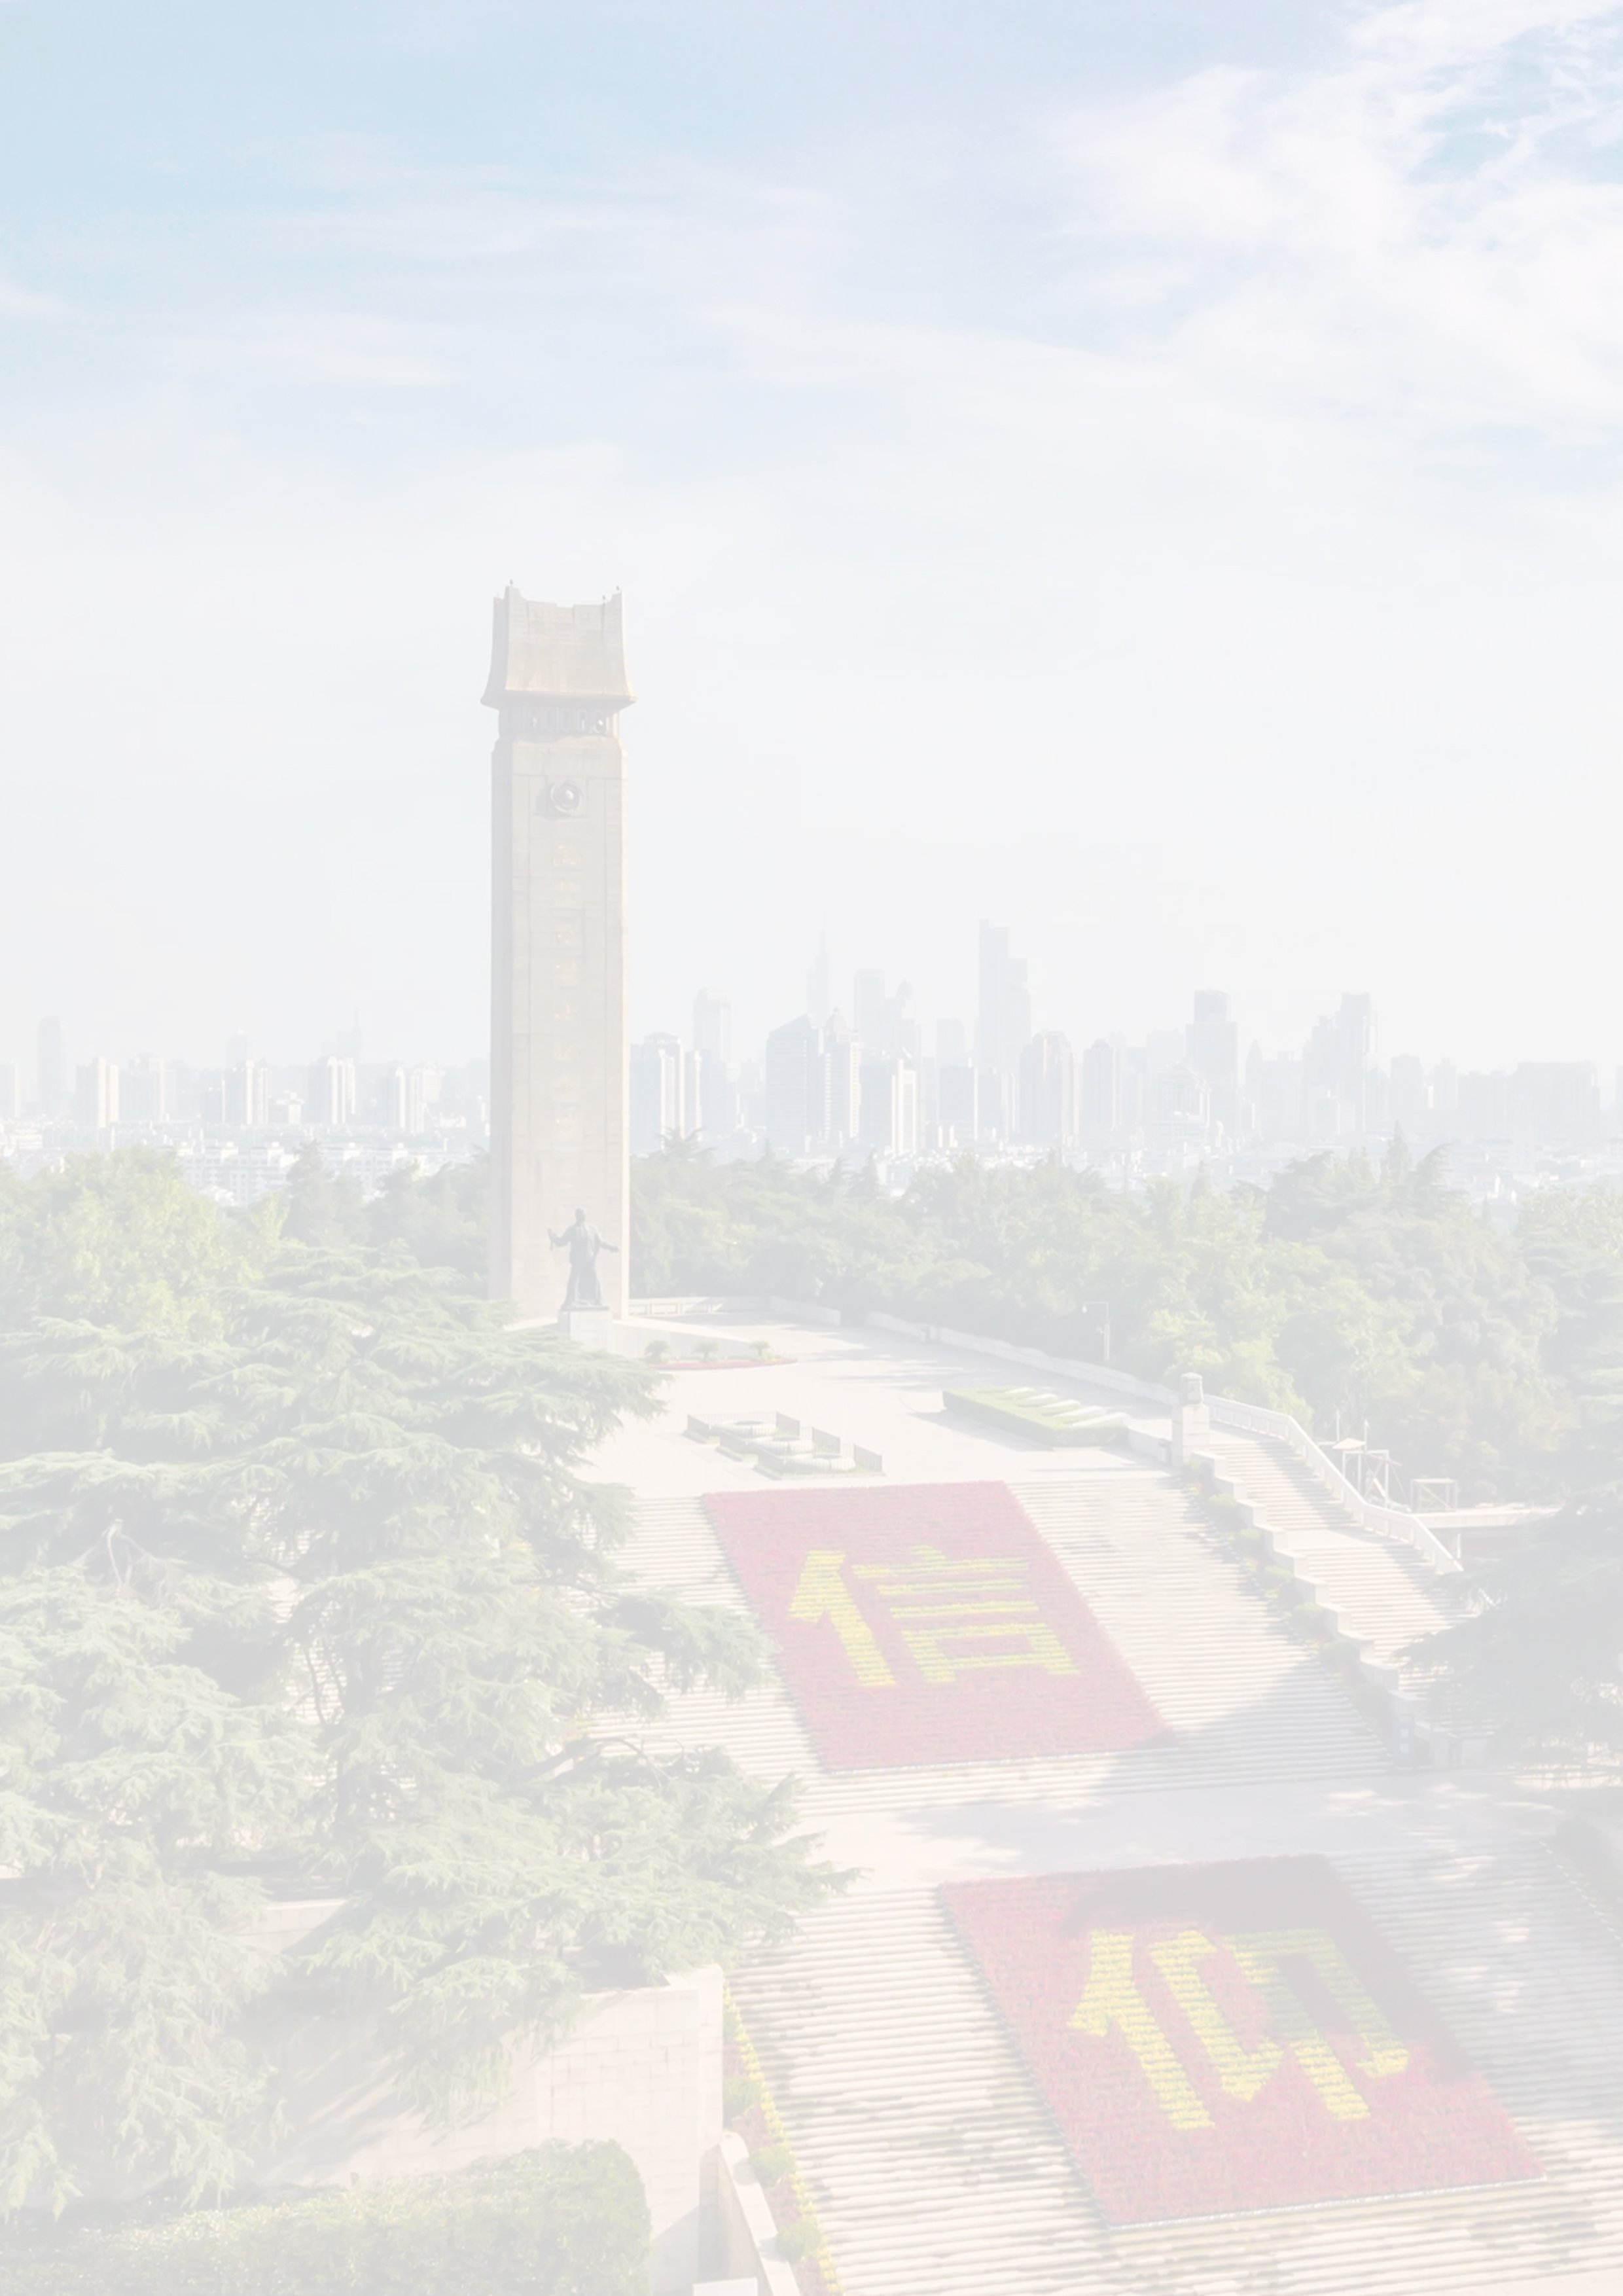
\includegraphics[width=1.25\paperwidth, height=1.2\paperwidth, 
	keepaspectratio]{Figures/背景.jpg}}}

\begin{document}

	\maketitle %有title的页面没有页眉页脚

	\tableofcontents

	这里填写摘要

	~ % ~可以当空行

	这里填写摘要这里填写摘要

	~

	这里填写摘要

	\vspace{7cm} %一般用在调整图片位置时。可以加空行使图片之间错开,或者图片和文字之间

	这里填写摘要这里填写摘要这里填写摘要这里填写摘要

	\begin{lstlisting} [language=c++]
		int main(int argc, char ** argv) 
		{ 

			printf("Hello world! \n"); 

			return 0; 
		} 
		\end{lstlisting}

	\newpage

	\section{一级标题}

	\begin{flushleft}
	左对齐
	\end{flushleft}

	\newpage

	\subsection{二级标题}

	\begin{flushright}
	右对齐
	\end{flushright}

	\subsubsection{三级标题}

	\begin{center}
	居中
	\end{center}

	\textbf{加粗}

	\textit{斜体}

	\underline{下划线}

	测试一下首行缩进测试一下首行缩进测试一下首行缩进测试一下首行缩进
	测试一下首行缩进测试一下首行缩进测试一下首行缩进测试一下首行缩进
	测试一下首行缩进测试一下首行缩进测试一下首行缩进测试一下首行缩进
	测试一下首行缩进测试一下首行缩进测试一下首行缩进测试一下首行缩进

	测试一下首行缩进测试一下首行缩进测试一下首行缩进测试一下首行缩进
	测试一下首行缩进测试一下首行缩进测试一下首行缩进测试一下首行缩进
	测试一下首行缩进测试一下首行缩进测试一下首行缩进测试一下首行缩进

	\begin{figure}[hbt]
		\centering
		
\includegraphics[width=2cm]{Ali.jpg}
		\caption{this is Ali}
	\end{figure}

	\begin{table}[htbp]
		\centering
		\caption{ACO算法与仅对ACO算法的量化策略进行修改得到的压缩效果对比}
		\begin{tabular}{cccc}
		\cline{1-4} %用于局部的划线
		\multirow{2}{*}{\textbf{Run ID}} & \multirow{2}{*}{\textbf{Dimension}}     & \multicolumn{2}{c}{\textbf{Compression Rate}} \\
						  &                       &   ACO        &   quan\_modified       \\ \cline{1-4}
			 ERR174324             & \multicolumn{1}{c|}{8998$\times$96} &   44.2\%        &    27.9\%      \\
			   ERR174331           & \multicolumn{1}{c|}{8998$\times$96} &    44.0\%       &   27.5\%       \\
			   ERR2438054          & \multicolumn{1}{c|}{5998$\times$146} &     37.7\%      &   36.6\%       \\ \cline{1-4}
		\end{tabular}
	\end{table}



\end{document}